\documentclass[12pt, journal]{IEEEtran}
\usepackage[utf8]{inputenc}   % ¡AHORA SÍ! Permite tildes y eñes directas desde el teclado
\usepackage[T1]{fontenc}       % Codificación de fuente para acentos y guionado en español
\usepackage[spanish]{babel}   % Idioma español
\usepackage{hyperref}         % Hipervínculos
\usepackage{graphicx}         % Manejo de imágenes
\usepackage{float}            % Control de posición de figuras [H]
\usepackage{gensymb}          % Símbolos genéricos (como grados °C)
\usepackage{amsmath}          % Fórmulas matemáticas optimizadas
\usepackage{tikz}             % Creación de gráficos
\usepackage{pgfplots}         % Creación de gráficas avanzadas
\usepackage{pgfplotstable}    % Regresión lineal integrada
\pgfplotsset{compat=1.18}     % Asegura compatibilidad de pgfplots para evitar warnings

\begin{document}

	% ==========================================
	% TÍTULO DEL REPORTE
	% ==========================================
	\title{ Resistencia dinámica de fuerzas viscosas  \\}

	\author{\IEEEauthorblockN{Jennifer Ovalle - Edson Pereira - Carlos Mogollón}
		\IEEEauthorblockA{\\ FABIQ $-$ FISICC\\
			Universidad Galileo\\
			Guatemala, Guatemala}}

	\maketitle

	% ==========================================
	% RESUMEN (ABSTRACT)
	% ==========================================
	\begin{abstract}
		Este experimento se realizó para implementar modelos matemáticos basados en ecuaciones diferenciales ordinarias (EDO) para lograr describir un fenómeno físico.
		Dicho fenómeno fue el de la resistencia dinámica de las fuerzas viscosas, en este caso se analiza el comportamiento de una pelota y un globo al dejarlas caer como caída libre desde un sexto y primer nivel respectivamente (esto con la idea de que alcancen sus velocidades terminales),
		con el fin de observar sus comportamientos a través del aire como fluido viscoso. Se graban ambos videos de las dos caídas, se guardan los datos posición-tiempo y luego se procesan en Tracker para poder graficar la curva velocidad vs tiempo.
		Se descubre que calcular el coeficiente de viscosidad de manera exacta (ya sea por cálculos teóricos, la app o el ajuste de IA) no fue posible, ya que en cada uno de los métodos usados siempre hubieron otros factores que impedía encontrar un solo valor de k exacto.
	\end{abstract}

	% ==========================================
	% INTRODUCCIÓN
	% ==========================================
	\section{Introducción}
		Se conoce como resistencia dinámica de una fuerza viscosa a la oposición que presenta el fluido en dirección opuesta a la fuerza aplicada para atravesar dicho fluido.
		Para describir este fenómeno físico se usó un modelo matemático basado en la ecuación diferencial ordinaria (EDO), siendo un modelo de una caída con resistencia del aire:
		$$m\,v' = m\,g - k\,v \quad\Longrightarrow\quad v' = g - \frac{k}{m}\,v$$
		Físicamente, el peso $mg$ acelera el cuerpo, la resistencia $kv$ lo frena, y esa resistencia crece con la velocidad. Por eso la velocidad se acerca a un valor límite, la velocidad terminal $v_{\infty} = mg/k$.
		\\ Este modelo sí tiene solución exacta:
		$$v(t) = \frac{mg}{k}\left(1 - e^{-kt/m}\right) + v_0\,e^{-kt/m}$$

		Viendo que se tiene una solución para el modelo, se quiso encontrar el valor de k que representa el coeficiente de viscosidad del fluido. Por medio de:
		datos experimentales, simulación usando el método Runge-Kutta y un ajuste por IA.
		\\ Entre la pelota y el globo, es probable que la pelota muestre resultados más fiables que el globo, debido a que el globo al ser tan ligero
		al momento de realizar el experimento se desviaba con facilidad a diferencia de la pelota, por lo que los datos del globo presentarán un error más grande.

	% ==========================================
	% PROCEDIMIENTO
	% ==========================================
	\section{Procedimiento}
	Breve descripción macroscópica de cómo se montó el experimento en el laboratorio o en casa.

	\subsection{Materiales y Equipamiento}
	\begin{itemize}
		\item \textbf{Pelota:} Se usó una pelota de fútbol mediana de masa 0.443kg.
		\item \textbf{Globo:} Un globo normal, de masa 0.002kg
		\item \textbf{(Software) Tracker:} Para facilitar la toma de datos, se usó tracker que cálcula y gráfica automáticamente solo con el video.
		\item \textbf{(Software) VsCode:} Para poder editar el reporte .tex (Latex), crear la app y el ajuste de IA (Python)
		\item \textbf{(Software) Github:} Se usó como repositorio general del proyecto completo, para que los 3 integrantes pudiesen subir y estar actualizados con los archivos del proyecto.
		\item \textbf{(IA) Claude:} Para hacer el ajuste con IA y ayuda con la app.
	\end{itemize}
	\subsection{Diagrama de Configuración del Laboratorio}

	\begin{figure}[H]
		\centering
		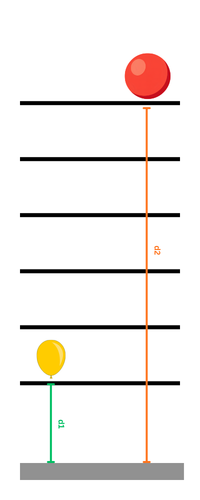
\includegraphics[width=10em]{Media/d1.png}
		\caption{Configuración de globo y pelota en función de los niveles del edificio de la Universidad Galileo.}
		\label{fig:montaje}
	\end{figure}


	\subsection{Pasos del Procedimiento}
	Se enumeran cronológicamente los pasos seguidos para la recolección de datos y la experimentación:
	\begin{enumerate}
		\item Medición y vertido del volumen idéntico de agua caliente en los contenedores.
		\item Toma de la temperatura ambiente inicial ($T_m$).
		\item Registro periódico de la temperatura del fluido a intervalos constantes de tiempo.
		\item Finalización del proceso al alcanzar la estabilización térmica.
	\end{enumerate}

	% ==========================================
	% RESULTADOS
	% ==========================================
	\section{Resultados}


	\subsection{Tabla de Datos Experimentales}

	\begin{table}[H]
		\centering
		\begin{tabular}{ccc|ccc}
			\hline
			\multicolumn{3}{c|}{\textbf{Globo} ($m = 0.002$~kg)} & \multicolumn{3}{c}{\textbf{Pelota} ($m = 0.443$~kg)} \\
			$t$ (s) & $y$ (m) & $v$ (m/s) & $t$ (s) & $y$ (m) & $v$ (m/s) \\
			\hline
			0.017 & $-0.012$ & 0.051 & 0.067 & $-0.099$ & 0.460 \\
			0.583 & $-0.278$ & 0.852 & 0.283 & $-0.308$ & 1.334 \\
			1.166 & $-0.673$ & 0.513 & 0.500 & $-0.707$ & 2.361 \\
			1.733 & $-0.975$ & 0.809 & 0.717 & $-1.285$ & 3.182 \\
			2.316 & $-1.603$ & 1.480 & 0.933 & $-2.075$ & 4.195 \\
			2.883 & $-2.361$ & 1.262 & 1.133 & $-3.077$ & 5.731 \\
			3.466 & $-2.963$ & 1.050 & 1.350 & $-4.477$ & 7.630 \\
			4.032 & $-3.590$ & 0.872 & 1.567 & $-6.399$ & 9.794 \\
			4.616 & $-4.267$ & 1.423 & 1.783 & $-8.969$ & 14.045 \\
			5.182 & $-5.217$ & 1.766 & 2.000 & $-12.630$ & 15.488 \\
			\hline
		\end{tabular}
		\caption{NOTA: Esta tabla está truncada.}
	\end{table}

	\subsection{Gráficas y Ajuste del Modelo}

	\begin{figure}[H]
		\centering
		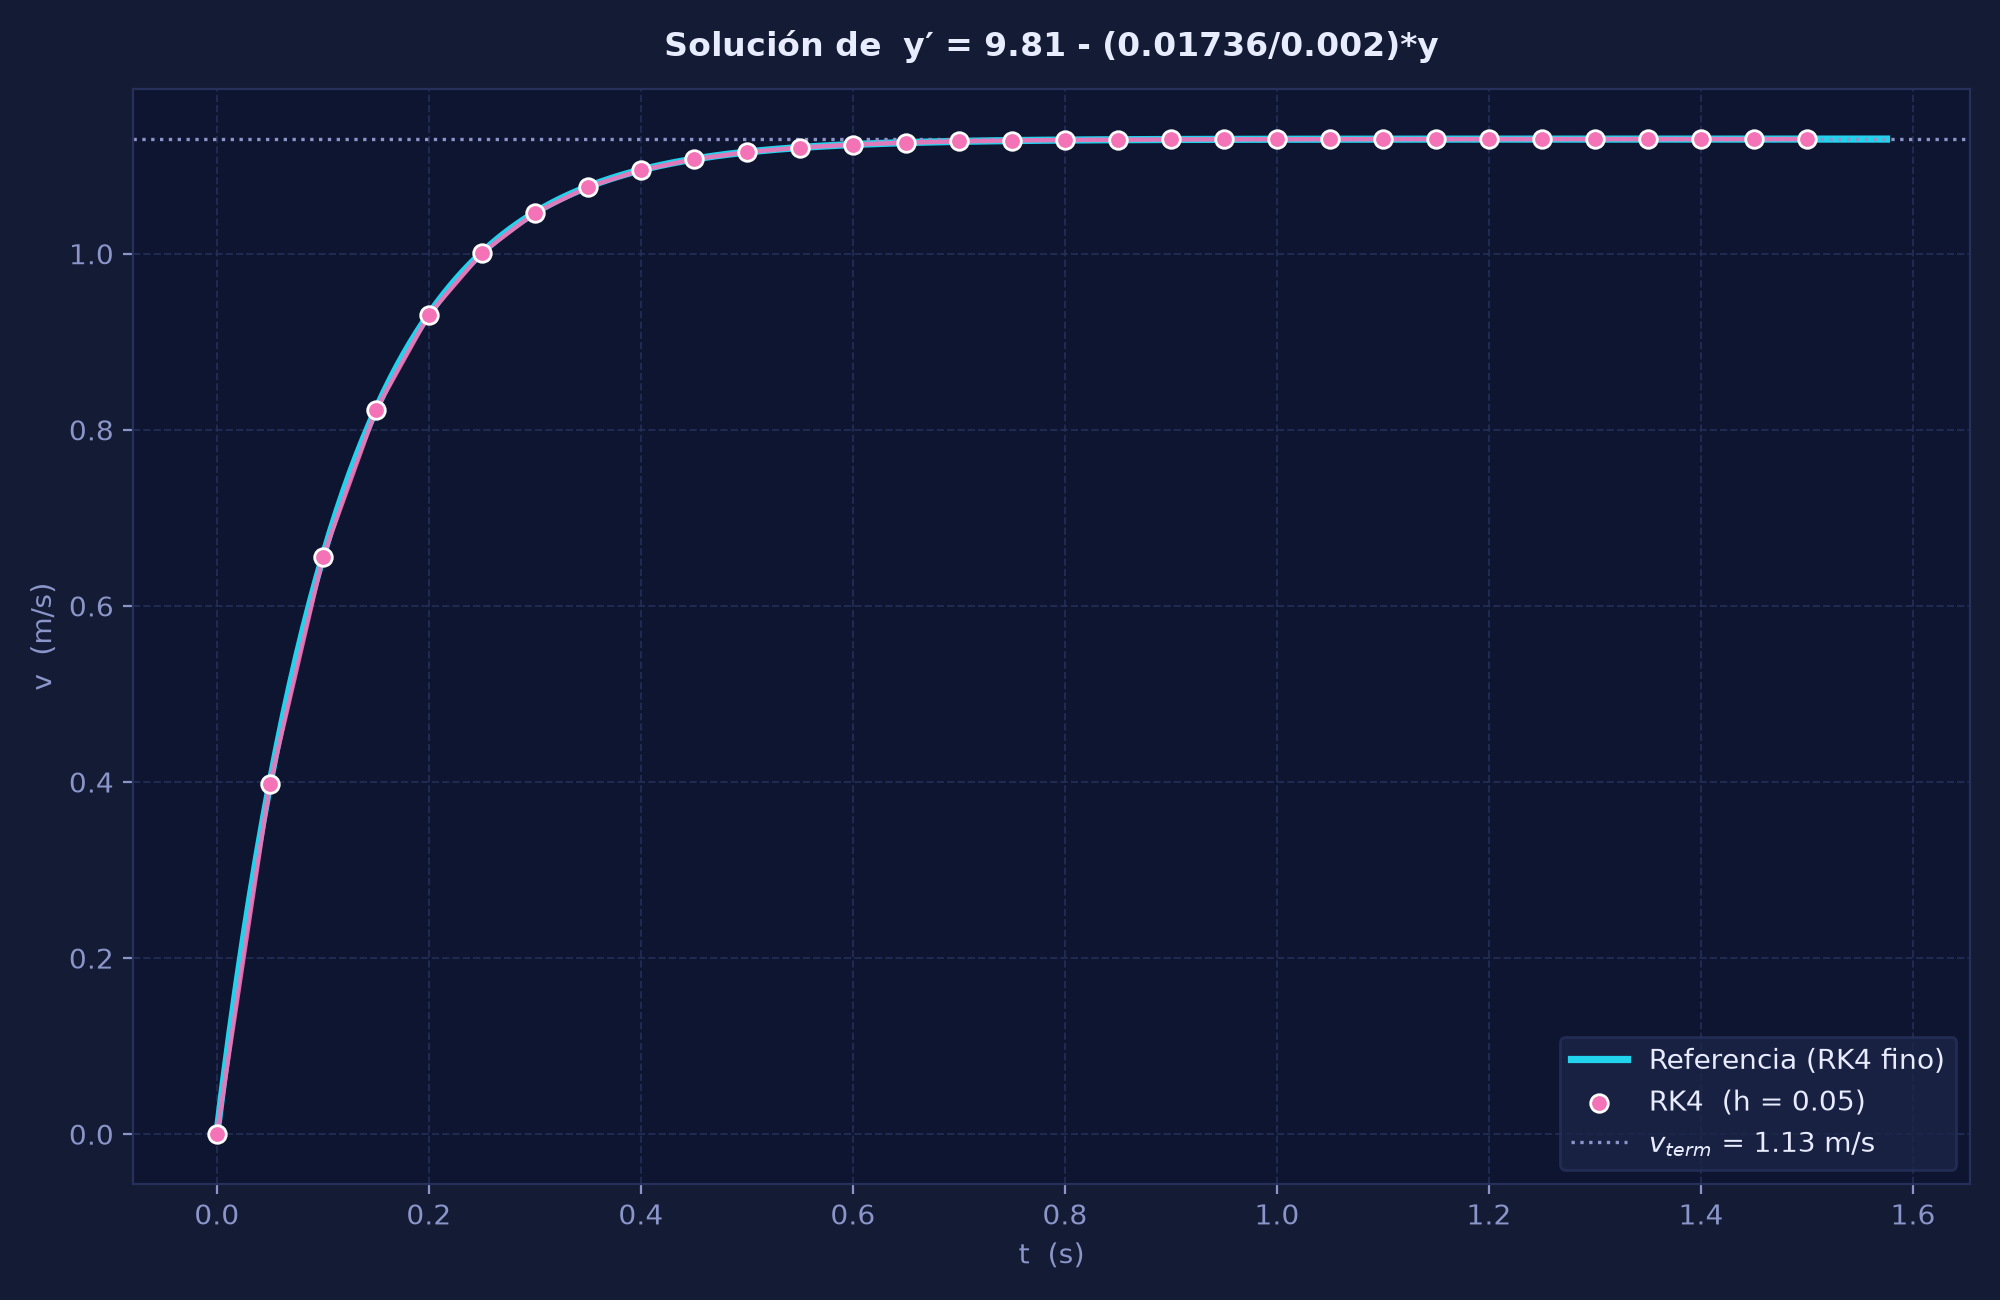
\includegraphics[width=\columnwidth]{Media/Kutta-globo.png}
		\caption{Solución numérica por RK4 para el globo.}
		\label{fig:rk4-globo}
	\end{figure}

	\begin{figure}[H]
		\centering
		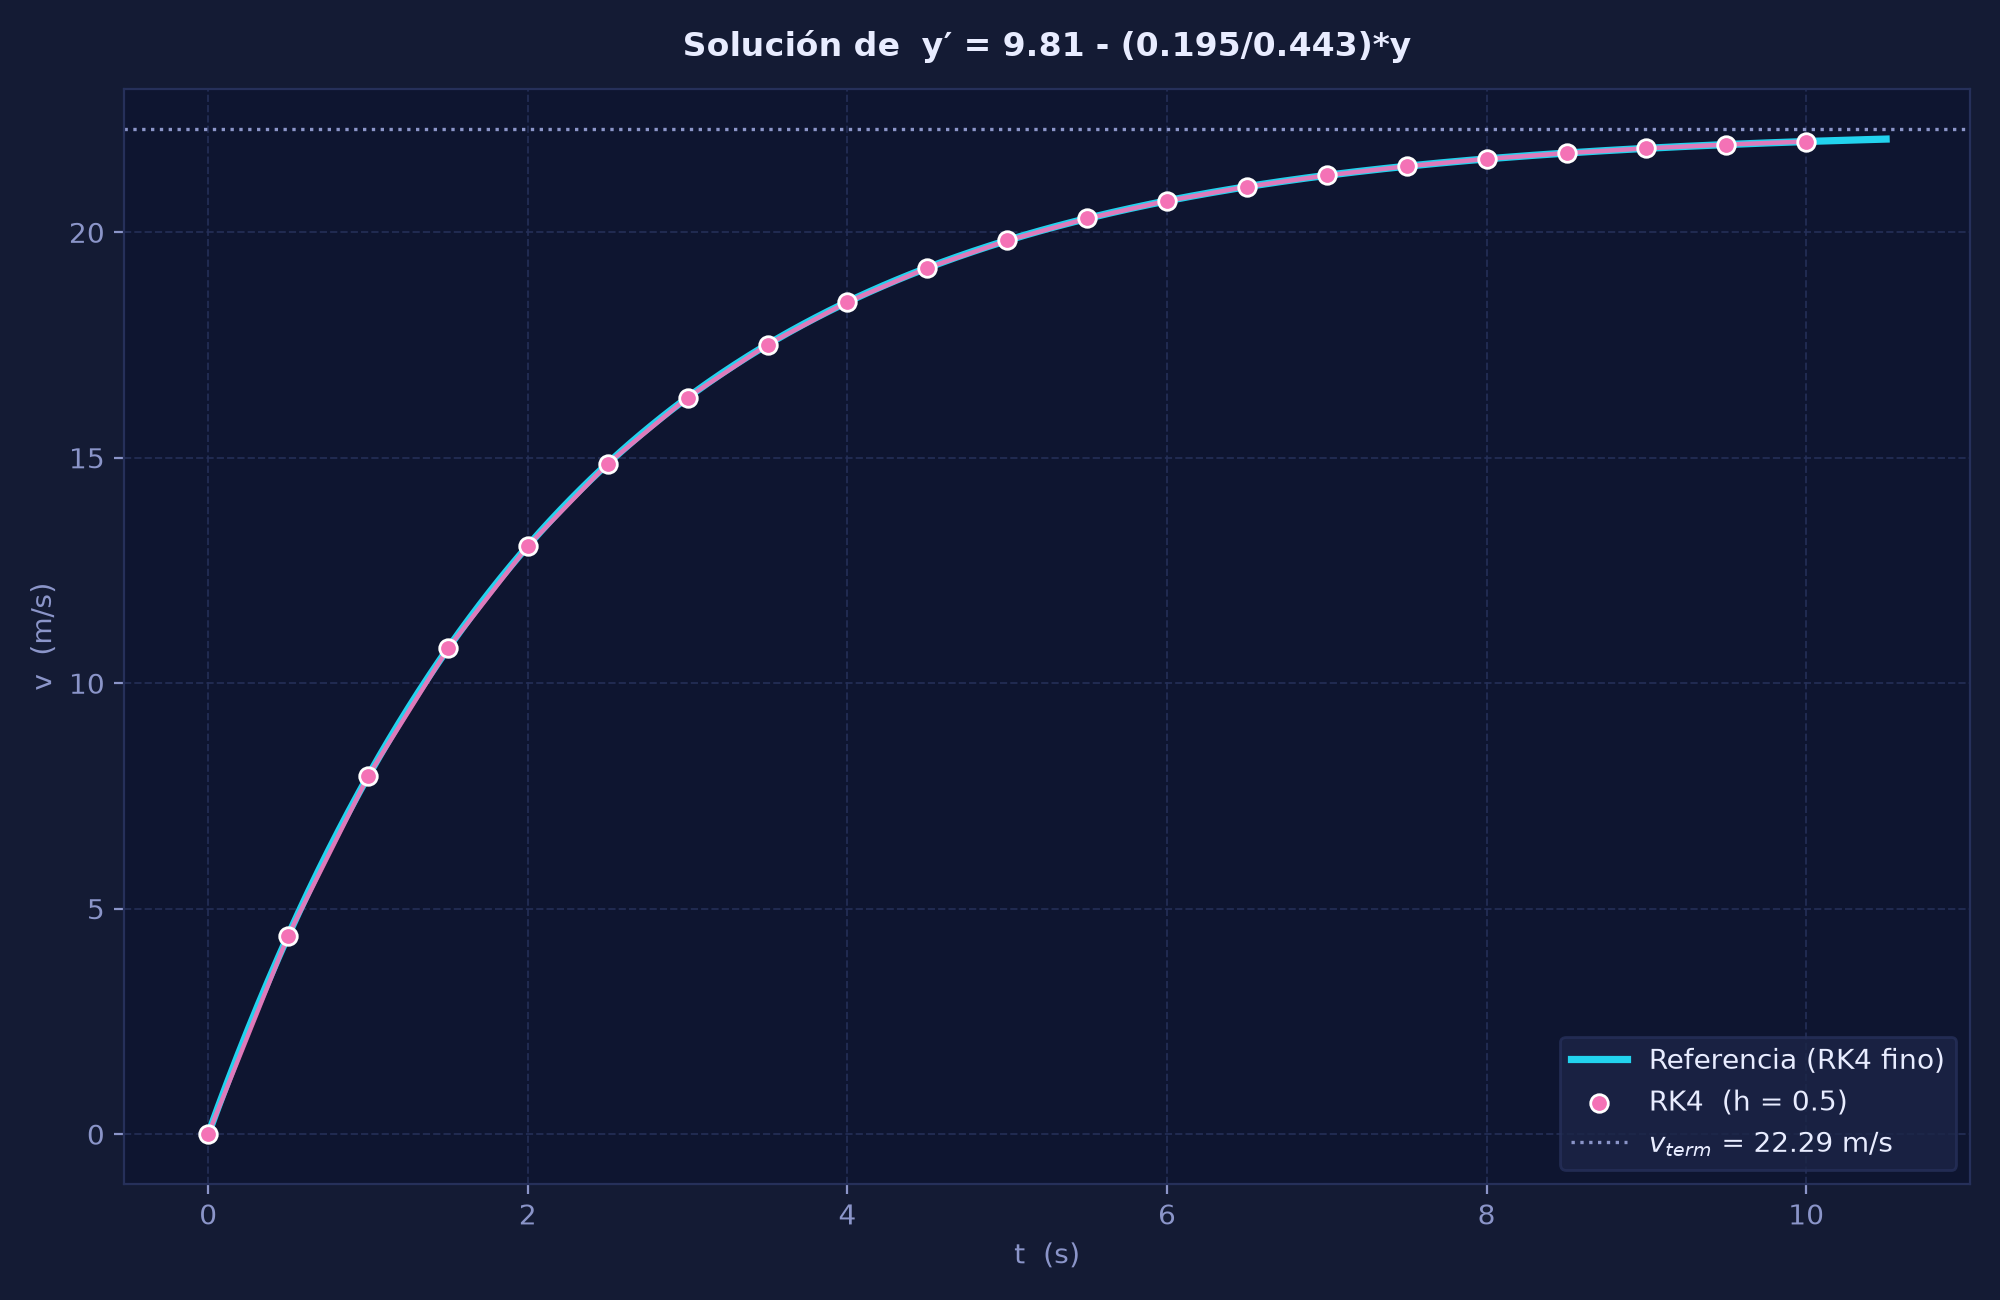
\includegraphics[width=\columnwidth]{Media/Kutta-pelota.png}
		\caption{Solución numérica por RK4 para la pelota.}
		\label{fig:rk4-pelota}
	\end{figure}

	% ==========================================
	% DISCUSIÓN / ANÁLISIS
	% ==========================================
	\section{Discusión / Análisis}

	\subsection{Resolución Analítica de la EDO}
	Tomando en cuenta el modelo propuesto en la introducción, tenemos la siguiente Ecuación Diferencial.
	\begin{equation}
        m\,\frac{dv}{dt} = mg - kv
	\end{equation}
	donde $m$ es la masa del objeto en caida libre y $k$ es el coeficiente de arrastre.
	Esta es una \textbf{EDO Separable}, entonces podemos reorganizar sus terminos:
	\begin{equation}
        \frac{v'}{mg - kv} = \frac{1}{m}
	\end{equation}
	Integrando ambos lados respecto a t:
	\begin{equation}
        -\frac{1}{k}\ln\left|mg - kv\right| = \frac{t}{m} + C
	\end{equation}
	Despejando $v$ de la expresión:
	\begin{equation}
        v(t) = \frac{mg}{k} + C\,e^{-\tfrac{k}{m}t}
	\end{equation}
	Esta de aqui es la  \textbf{solución general de la EDO}. Podemos aplicar la condición $v(0) = v_0$ para despejar $C$:
	\begin{equation}
        v_0 = \frac{mg}{k} + C \quad\Rightarrow\quad C = v_0 - \frac{mg}{k}
	\end{equation}
	De aqui se obtiene la siguiente \textbf{solución particular para la EDO}:
	\begin{equation}
        \boxed{v(t) = \frac{mg}{k}\!\left(1 - e^{-\tfrac{k}{m}t}\right) + v_0\,e^{-\tfrac{k}{m}t}}
        \label{eq:sol_particular}
	\end{equation}
	Si analizamos esta expresión cuando $t \to \infty$, el término exponencial se anula y la velocidad converge a la expresión para la \textbf{velocidad terminal}:
	\begin{equation}
        \lim_{t\to\infty} v(t) = \frac{mg}{k}
	\end{equation}


	\subsection{Cálculo analítico de la constante \boldmath$k$}

	Con la solución particular de la EDO \eqref{eq:sol_particular}, partimos del supuesto que empezamos en reposo, osea  $v_0 \approx 0$:
	\begin{equation}
        v(t) = \frac{mg}{k}\!\left(1 - e^{-\tfrac{k}{m}t}\right)
	\end{equation}
	Si analizamos esta expresión a medida que $t \to \infty$ la exponencial se anula y $v_t = mg/k$.
	Si ahora despejamos para el coeficiente \boldmath$k$:

	\begin{equation}
    k = \frac{mg}{v_t}
    \label{eq:k_analitico}
	\end{equation}
	Para el \textbf{globo} ($m = 0{,}002~\text{kg}$), el último dato que tenemos de nuestro experimento
	($t = 5{,}182~\text{s}$, $v = 1{,}766~\text{m/s}$) se toma para una aproximación de $v_t$:

	\begin{align}
        k_{\text{globo}} &= \frac{(0{,}002~\text{kg})(9{,}81~\text{m/s}^2)}{1{,}766~\text{m/s}} \notag \\
        &\approx 0{,}0111~\frac{\text{N}\cdot\text{s}}{\text{m}}
        \label{eq:k_globo}
	\end{align}

	Para la \textbf{pelota} ($m = 0{,}443~\text{kg}$), los datos disponibles
	($t_{\max} = 2{,}0~\text{s}$, $v_{\max} \approx 15{,}5~\text{m/s}$) no alcanzan
	la velocidad terminal, por lo que la ecuación~\eqref{eq:k_analitico} no aplica.
	Para este caso, vamos a calcular $k$ haciendo uso de la expresión de caida libre $v=gt$:

	\begin{align}
        v(2{,}0) &= 9{,}81 \times 2{,}0 = 19{,}62~\text{m/s} \notag \\
        \Delta v &= 19{,}62 - 15{,}49 = 4{,}13~\text{m/s} \notag \\
        k_{\text{pelota}} &\approx \frac{m\,\Delta v}{t_{\max}\,\bar{v}}
        = \frac{(0{,}443)(4{,}13)}{(2{,}0)(15{,}49)}
        \approx 0{,}059~\frac{\text{N}\cdot\text{s}}{\text{m}}
        \label{eq:k_pelota}
	\end{align}

	% ==========================================
	% CONCLUSIÓN
	% ==========================================
	\section{Conclusión}
	Esta sección incluye un cierre conciso basado en la evidencia de los resultados y cómo se relacionan con los objetivos iniciales. Se debe destacar de manera clara qué se aprendió acerca del modelado por ecuaciones diferenciales en procesos de transferencia de calor reales.

	% ==========================================
	% REFERENCIAS
	% ==========================================
	\begin{thebibliography}{1}

		\bibitem{Zill}
		D.~G.~Zill, \emph{Ecuaciones diferenciales con aplicaciones de modelado}, 11a ed. Cengage Learning, 2018.

		\bibitem{Incropera}
		F.~P.~Incropera, D.~P.~DeWitt, \emph{Fundamentos de transferencia de calor}, 4a ed. México: Prentice Hall, 1999.

		\bibitem{LabWrite}
		M.~Carter, E.~Weiebe, and M.~Ferzli, \emph{LabWrite}, \url{https://www.ncsu.edu/labwrite/index_labwrite.htm}, NC~State~University, 2004.

	\end{thebibliography}

\end{document}
